% Options for packages loaded elsewhere
\PassOptionsToPackage{unicode}{hyperref}
\PassOptionsToPackage{hyphens}{url}
\PassOptionsToPackage{dvipsnames,svgnames,x11names}{xcolor}
%
\documentclass[
  8pt,
  ignorenonframetext,
  aspectratio=169]{beamer}
\title{Crash course: Geospatial Datavisualisering}
\author{Jeppe Vierø}
\date{\today}

\usepackage{pgfpages}
\setbeamertemplate{caption}[numbered]
\setbeamertemplate{caption label separator}{: }
\setbeamercolor{caption name}{fg=normal text.fg}
\beamertemplatenavigationsymbolsempty
% Prevent slide breaks in the middle of a paragraph
\widowpenalties 1 10000
\raggedbottom
\setbeamertemplate{part page}{
  \centering
  \begin{beamercolorbox}[sep=16pt,center]{part title}
    \usebeamerfont{part title}\insertpart\par
  \end{beamercolorbox}
}
\setbeamertemplate{section page}{
  \centering
  \begin{beamercolorbox}[sep=12pt,center]{part title}
    \usebeamerfont{section title}\insertsection\par
  \end{beamercolorbox}
}
\setbeamertemplate{subsection page}{
  \centering
  \begin{beamercolorbox}[sep=8pt,center]{part title}
    \usebeamerfont{subsection title}\insertsubsection\par
  \end{beamercolorbox}
}
\AtBeginPart{
  \frame{\partpage}
}
\AtBeginSection{
  \ifbibliography
  \else
    \frame{\sectionpage}
  \fi
}
\AtBeginSubsection{
  \frame{\subsectionpage}
}
\usepackage{amsmath,amssymb}
\usepackage{lmodern}
\usepackage{iftex}
\ifPDFTeX
  \usepackage[T1]{fontenc}
  \usepackage[utf8]{inputenc}
  \usepackage{textcomp} % provide euro and other symbols
\else % if luatex or xetex
  \usepackage{unicode-math}
  \defaultfontfeatures{Scale=MatchLowercase}
  \defaultfontfeatures[\rmfamily]{Ligatures=TeX,Scale=1}
\fi
\usetheme[]{CambridgeUS}
% Use upquote if available, for straight quotes in verbatim environments
\IfFileExists{upquote.sty}{\usepackage{upquote}}{}
\IfFileExists{microtype.sty}{% use microtype if available
  \usepackage[]{microtype}
  \UseMicrotypeSet[protrusion]{basicmath} % disable protrusion for tt fonts
}{}
\makeatletter
\@ifundefined{KOMAClassName}{% if non-KOMA class
  \IfFileExists{parskip.sty}{%
    \usepackage{parskip}
  }{% else
    \setlength{\parindent}{0pt}
    \setlength{\parskip}{6pt plus 2pt minus 1pt}}
}{% if KOMA class
  \KOMAoptions{parskip=half}}
\makeatother
\usepackage{xcolor}
\IfFileExists{xurl.sty}{\usepackage{xurl}}{} % add URL line breaks if available
\IfFileExists{bookmark.sty}{\usepackage{bookmark}}{\usepackage{hyperref}}
\hypersetup{
  pdftitle={Crash course: Geospatial Datavisualisering},
  pdfauthor={Jeppe Vierø},
  colorlinks=true,
  linkcolor={Maroon},
  filecolor={Maroon},
  citecolor={Blue},
  urlcolor={blue},
  pdfcreator={LaTeX via pandoc}}
\urlstyle{same} % disable monospaced font for URLs
\newif\ifbibliography
\usepackage{color}
\usepackage{fancyvrb}
\newcommand{\VerbBar}{|}
\newcommand{\VERB}{\Verb[commandchars=\\\{\}]}
\DefineVerbatimEnvironment{Highlighting}{Verbatim}{commandchars=\\\{\}}
% Add ',fontsize=\small' for more characters per line
\newenvironment{Shaded}{}{}
\newcommand{\AlertTok}[1]{\textcolor[rgb]{1.00,0.00,0.00}{\textbf{#1}}}
\newcommand{\AnnotationTok}[1]{\textcolor[rgb]{0.38,0.63,0.69}{\textbf{\textit{#1}}}}
\newcommand{\AttributeTok}[1]{\textcolor[rgb]{0.49,0.56,0.16}{#1}}
\newcommand{\BaseNTok}[1]{\textcolor[rgb]{0.25,0.63,0.44}{#1}}
\newcommand{\BuiltInTok}[1]{#1}
\newcommand{\CharTok}[1]{\textcolor[rgb]{0.25,0.44,0.63}{#1}}
\newcommand{\CommentTok}[1]{\textcolor[rgb]{0.38,0.63,0.69}{\textit{#1}}}
\newcommand{\CommentVarTok}[1]{\textcolor[rgb]{0.38,0.63,0.69}{\textbf{\textit{#1}}}}
\newcommand{\ConstantTok}[1]{\textcolor[rgb]{0.53,0.00,0.00}{#1}}
\newcommand{\ControlFlowTok}[1]{\textcolor[rgb]{0.00,0.44,0.13}{\textbf{#1}}}
\newcommand{\DataTypeTok}[1]{\textcolor[rgb]{0.56,0.13,0.00}{#1}}
\newcommand{\DecValTok}[1]{\textcolor[rgb]{0.25,0.63,0.44}{#1}}
\newcommand{\DocumentationTok}[1]{\textcolor[rgb]{0.73,0.13,0.13}{\textit{#1}}}
\newcommand{\ErrorTok}[1]{\textcolor[rgb]{1.00,0.00,0.00}{\textbf{#1}}}
\newcommand{\ExtensionTok}[1]{#1}
\newcommand{\FloatTok}[1]{\textcolor[rgb]{0.25,0.63,0.44}{#1}}
\newcommand{\FunctionTok}[1]{\textcolor[rgb]{0.02,0.16,0.49}{#1}}
\newcommand{\ImportTok}[1]{#1}
\newcommand{\InformationTok}[1]{\textcolor[rgb]{0.38,0.63,0.69}{\textbf{\textit{#1}}}}
\newcommand{\KeywordTok}[1]{\textcolor[rgb]{0.00,0.44,0.13}{\textbf{#1}}}
\newcommand{\NormalTok}[1]{#1}
\newcommand{\OperatorTok}[1]{\textcolor[rgb]{0.40,0.40,0.40}{#1}}
\newcommand{\OtherTok}[1]{\textcolor[rgb]{0.00,0.44,0.13}{#1}}
\newcommand{\PreprocessorTok}[1]{\textcolor[rgb]{0.74,0.48,0.00}{#1}}
\newcommand{\RegionMarkerTok}[1]{#1}
\newcommand{\SpecialCharTok}[1]{\textcolor[rgb]{0.25,0.44,0.63}{#1}}
\newcommand{\SpecialStringTok}[1]{\textcolor[rgb]{0.73,0.40,0.53}{#1}}
\newcommand{\StringTok}[1]{\textcolor[rgb]{0.25,0.44,0.63}{#1}}
\newcommand{\VariableTok}[1]{\textcolor[rgb]{0.10,0.09,0.49}{#1}}
\newcommand{\VerbatimStringTok}[1]{\textcolor[rgb]{0.25,0.44,0.63}{#1}}
\newcommand{\WarningTok}[1]{\textcolor[rgb]{0.38,0.63,0.69}{\textbf{\textit{#1}}}}
\usepackage{graphicx}
\makeatletter
\def\maxwidth{\ifdim\Gin@nat@width>\linewidth\linewidth\else\Gin@nat@width\fi}
\def\maxheight{\ifdim\Gin@nat@height>\textheight\textheight\else\Gin@nat@height\fi}
\makeatother
% Scale images if necessary, so that they will not overflow the page
% margins by default, and it is still possible to overwrite the defaults
% using explicit options in \includegraphics[width, height, ...]{}
\setkeys{Gin}{width=\maxwidth,height=\maxheight,keepaspectratio}
% Set default figure placement to htbp
\makeatletter
\def\fps@figure{htbp}
\makeatother
\setlength{\emergencystretch}{3em} % prevent overfull lines
\providecommand{\tightlist}{%
  \setlength{\itemsep}{0pt}\setlength{\parskip}{0pt}}
\setcounter{secnumdepth}{-\maxdimen} % remove section numbering
\newcommand{\columnsbegin}{\begin{columns}}
\newcommand{\columnsend}{\end{columns}}


\AtBeginSection{
   \frame{\sectionpage}
}

\makeatletter
\setbeamertemplate{section page}
{
  \begingroup
    \centering
%    {\usebeamerfont{section name}\usebeamercolor[fg]{section name}\sectionname~\insertsectionnumber}
    \vskip1em\par
    \begin{beamercolorbox}[sep=12pt,center,colsep=-4bp,rounded=true,shadow=\beamer@themerounded@shadow]{section title}
      \usebeamerfont{section title}\insertsection\par
    \end{beamercolorbox}
  \endgroup
}
\makeatother


\usepackage{hyperref}
\ifLuaTeX
  \usepackage{selnolig}  % disable illegal ligatures
\fi

\begin{document}
\frame{\titlepage}

\begin{frame}[allowframebreaks]
  \tableofcontents[hideallsubsections]
\end{frame}
\hypertarget{xx}{%
\section{xx}\label{xx}}

\hypertarget{introduktion}{%
\section{Introduktion}\label{introduktion}}

\begin{frame}{Motivation}
\protect\hypertarget{motivation}{}
\begin{figure}[H]
    \centering
    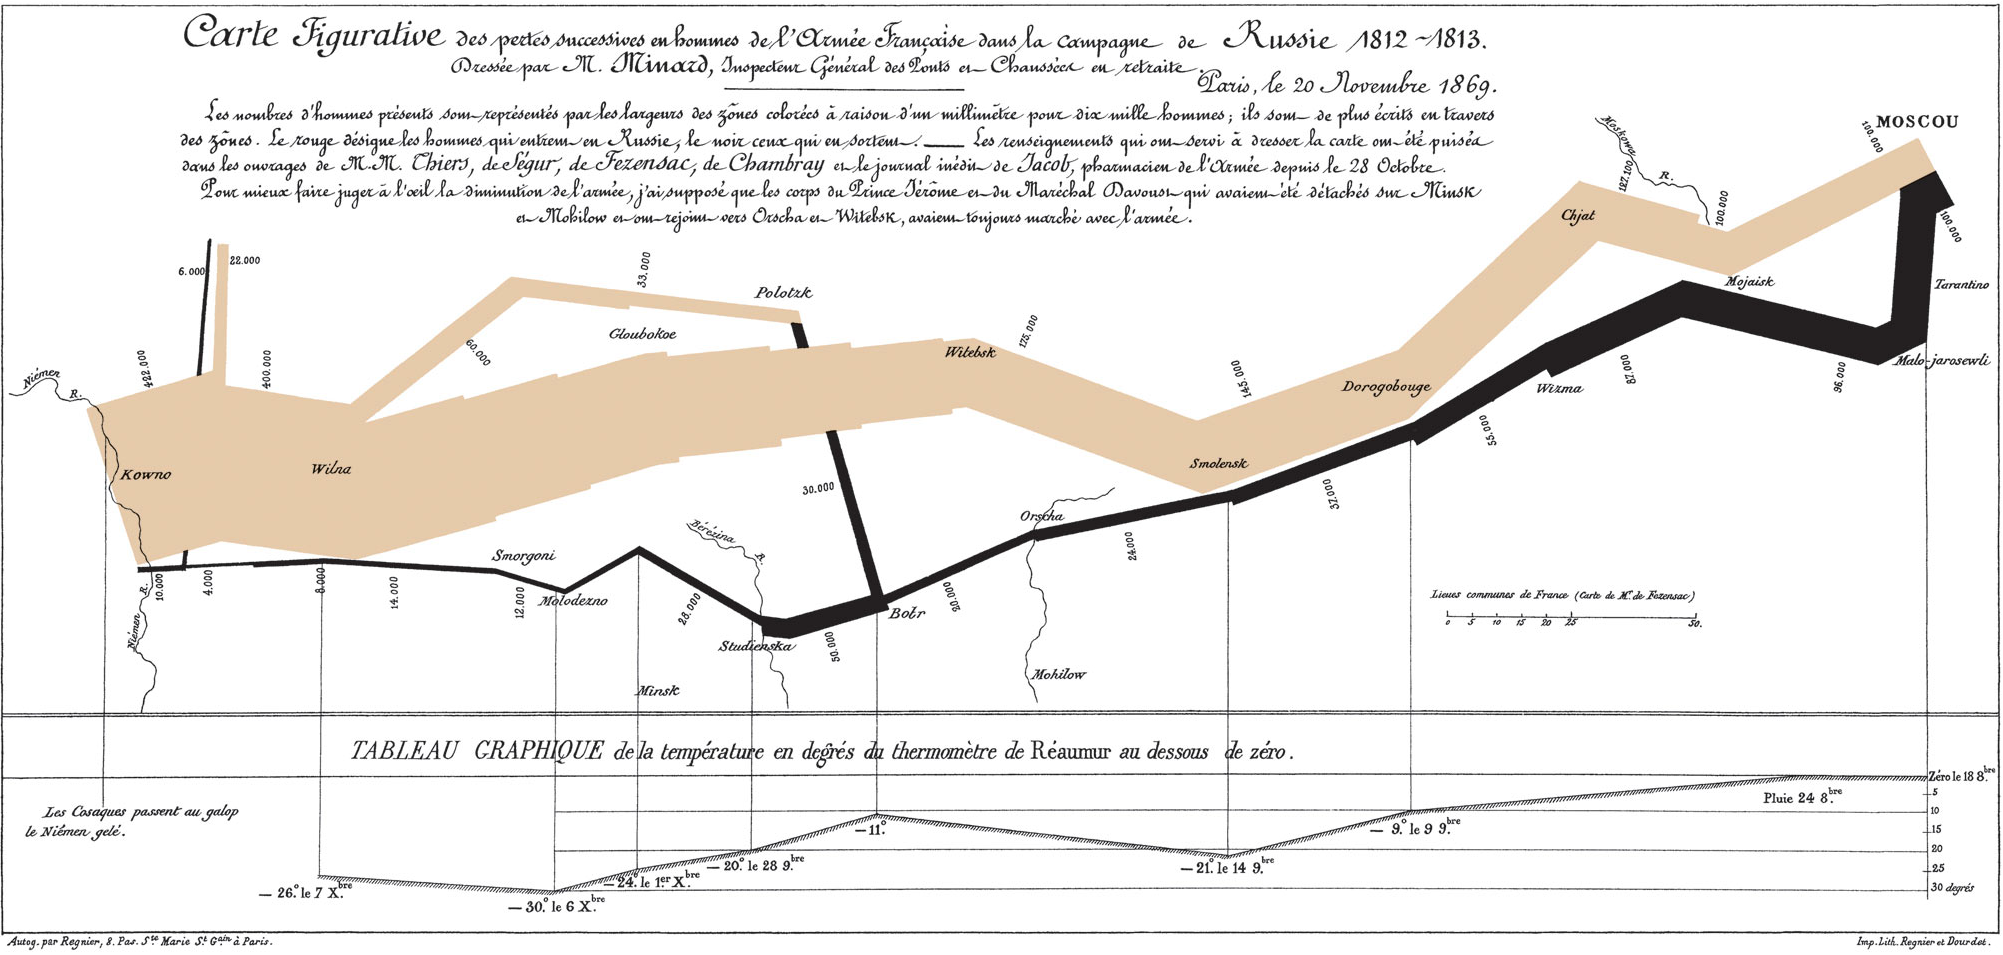
\includegraphics[width=.90\textwidth]{pictures/Minard.png}
\end{figure}
\end{frame}

\begin{frame}[fragile]{Afgrænsning}
\protect\hypertarget{afgruxe6nsning}{}
Jeg (regner med) at snakke \textbf{en del} om:

\begin{itemize}
\item
  Hvad \textbf{spatial} data er
\item
  Hvordan vi kan bruge spatiale datakilder til at \textbf{visualisere}
  andet data
\item
  Hvordan vi gør det i \texttt{R}
\end{itemize}

\bigskip

Jeg kommer \textbf{ikke} til at snakke (så meget) om:

\begin{itemize}
\item
  Datawrangling og -manipulation med geospatial data
\item
  Datavisualisering generelt
\end{itemize}
\end{frame}

\hypertarget{section}{%
\section{section}\label{section}}

\begin{frame}{section}
\end{frame}

\begin{frame}[fragile]{load}
\protect\hypertarget{load}{}
\begin{Shaded}
\begin{Highlighting}[]
\FunctionTok{library}\NormalTok{(tidyverse)}
\FunctionTok{library}\NormalTok{(janitor)}
\FunctionTok{library}\NormalTok{(sf)}
\FunctionTok{library}\NormalTok{(tmap)}
\FunctionTok{library}\NormalTok{(repinion)}

\CommentTok{\# Installér \{repinion\}, hvis I ikke har den:}
\CommentTok{\# devtools::install\_github("jvieroe/repinion")}
\end{Highlighting}
\end{Shaded}
\end{frame}

\begin{frame}[fragile]{xxxx}
\protect\hypertarget{xxxx}{}
xxx

\begin{Shaded}
\begin{Highlighting}[]
\NormalTok{rejser }\OtherTok{\textless{}{-}} \FunctionTok{readRDS}\NormalTok{(}\StringTok{"data/rejsekortdata.rds"}\NormalTok{)}
\FunctionTok{head}\NormalTok{(rejser, }\DecValTok{5}\NormalTok{)}
\end{Highlighting}
\end{Shaded}

\begin{verbatim}
## # A tibble: 5 x 3
##   count station             share
##   <int> <chr>               <dbl>
## 1  5875 Nørreport St.      0.0688
## 2  5875 Kongens Nytorv St. 0.0652
## 3  5875 København H        0.0482
## 4  5875 Trianglen St.      0.0480
## 5  5875 Frederiksberg St.  0.0476
\end{verbatim}
\end{frame}

\begin{frame}[fragile]{y}
\protect\hypertarget{y}{}
\columnsbegin
\column{.5\textwidth}

\begin{Shaded}
\begin{Highlighting}[]
\FunctionTok{plot}\NormalTok{(mtcars[, }\DecValTok{1}\SpecialCharTok{:}\DecValTok{3}\NormalTok{])}
\end{Highlighting}
\end{Shaded}

\column{.5\textwidth}

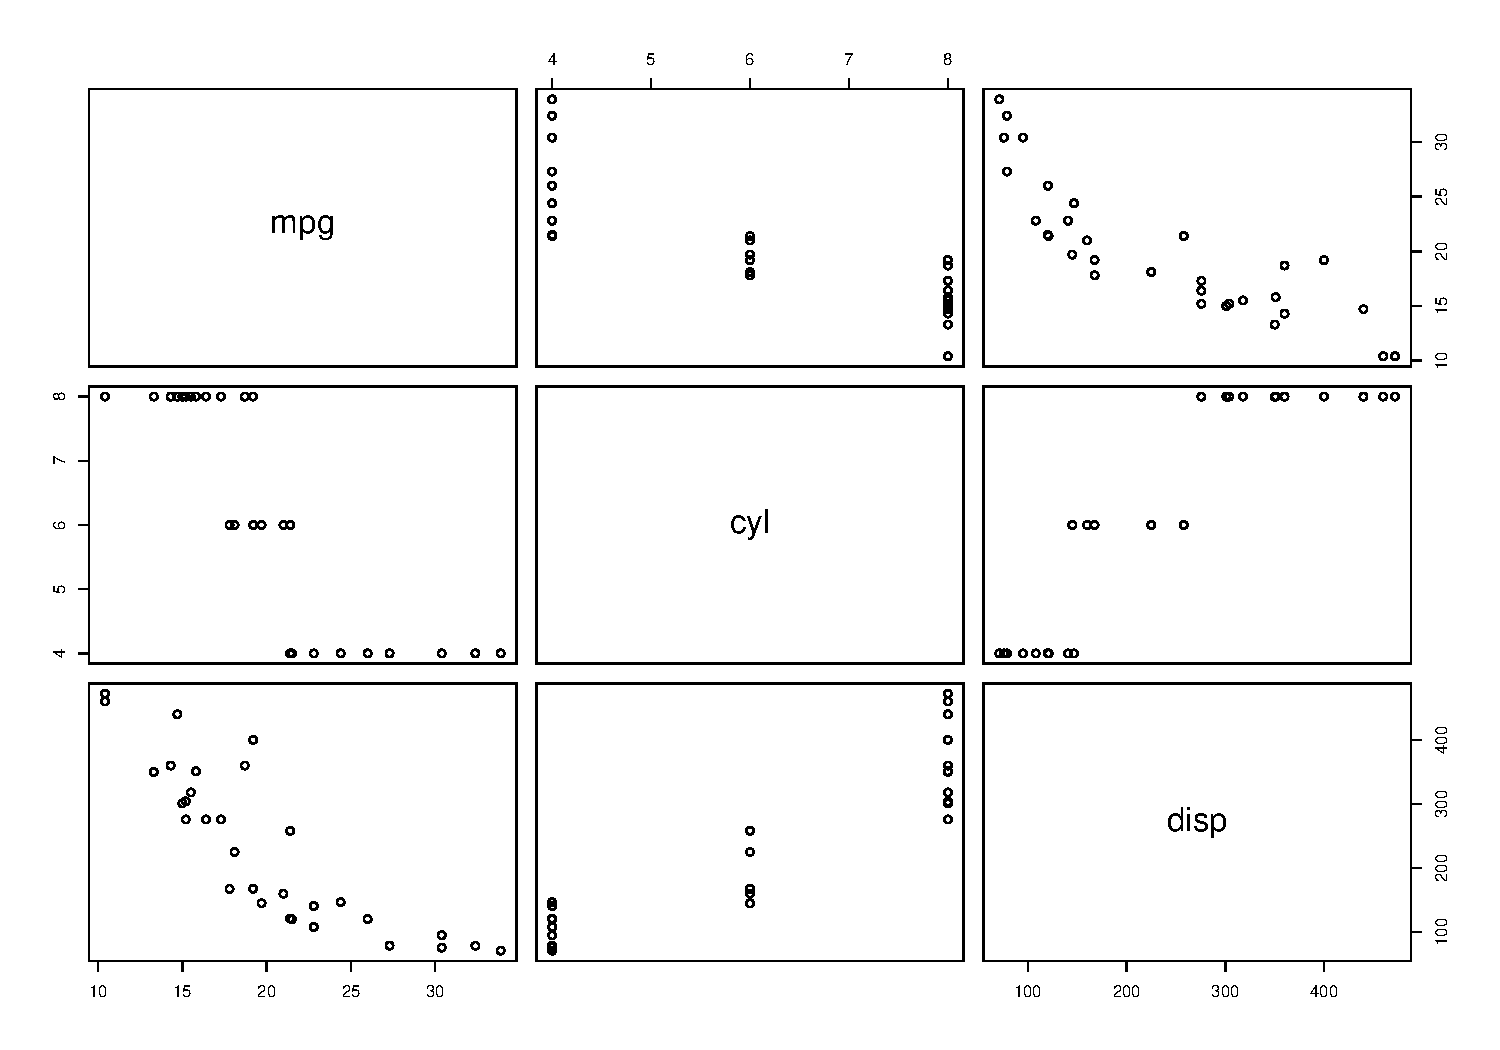
\includegraphics{crashcourse_slides_files/figure-beamer/unnamed-chunk-4-1.pdf}
\columnsend
\end{frame}

\hypertarget{datastrukturer}{%
\section{Datastrukturer}\label{datastrukturer}}

\begin{frame}{Need to know om geodata}
\protect\hypertarget{need-to-know-om-geodata}{}
text
\end{frame}

\begin{frame}{Typer af geodata}
\protect\hypertarget{typer-af-geodata}{}
Grundlæggende arbejder vi med \textbf{tre typer af geospatiale
datakilder}

Hver type har en (nogenlunde) parallel til graftyper, I er vant til at
arbejde med:

\bigskip

\begin{enumerate}
\tightlist
\item
  \textbf{Punkter}
\end{enumerate}

\begin{itemize}
\tightlist
\item
  Tænk på dem som almindelige \emph{punkter i et scatterplot}
\end{itemize}

\begin{enumerate}
\setcounter{enumi}{1}
\tightlist
\item
  \textbf{Linjer}
\end{enumerate}

\begin{itemize}
\tightlist
\item
  Tænk på dem som \emph{linjer i et linechart}
\end{itemize}

\begin{enumerate}
\setcounter{enumi}{2}
\tightlist
\item
  \textbf{Polygoner}
\end{enumerate}

\begin{itemize}
\tightlist
\item
  Her er parallelen ikke lige så tydelig
\item
  \ldots{} men i en data viz-kontekst kan I tænke på dem som
  \emph{søjler i et bar chart} (ish\ldots)
\end{itemize}
\end{frame}

\begin{frame}{(1) Punkter}
\protect\hypertarget{punkter}{}
\columnsbegin
\column{.4\textwidth}

\begin{itemize}
\item
  Punkter består af simple koordinater (x, y), der refererer til en
  specifik lokation
\item
  Punkter har ingen størrelse (og intet \emph{areal}), de er uendeligt
  små
\item
  Eksempler: byer, stationer, skoler osv.
\end{itemize}

\column{.6\textwidth}

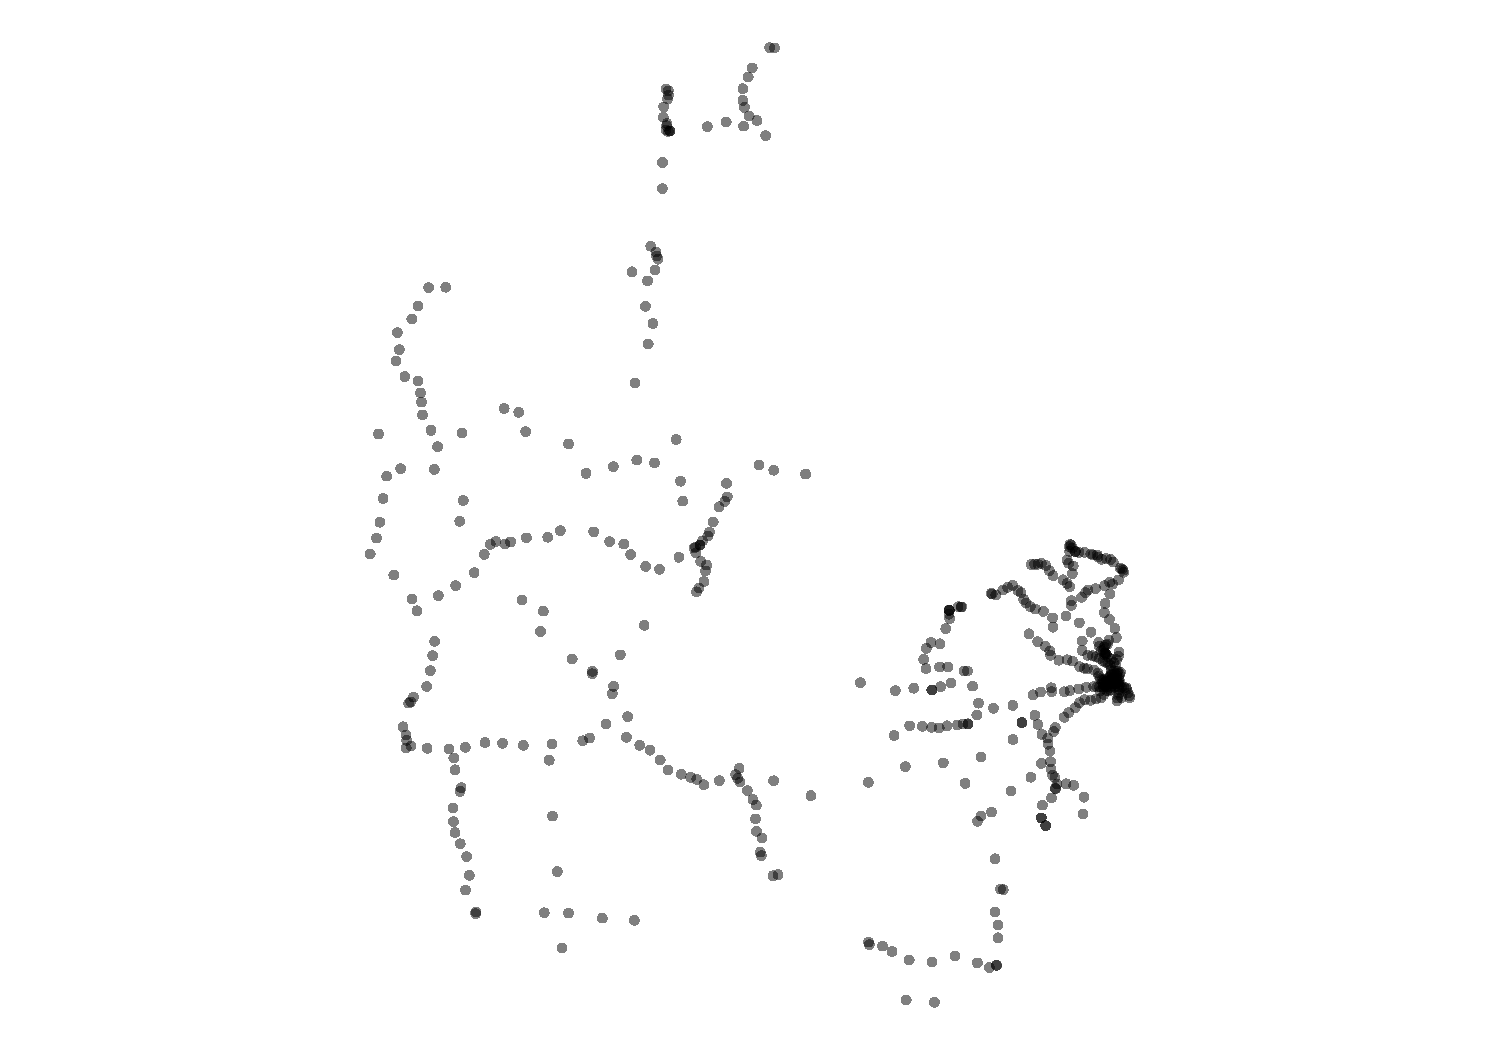
\includegraphics[width=1\linewidth]{crashcourse_slides_files/figure-beamer/unnamed-chunk-6-1}

\columnsend
\end{frame}

\begin{frame}{(2) Linjer}
\protect\hypertarget{linjer}{}
\columnsbegin
\column{.4\textwidth}

\begin{itemize}
\item
  Linjer består -- grundlæggende -- af punkter, der er kombineret til en
  \emph{linestring} vha. en defineret rækkefølge
\item
  Konstruktionen er sjældent noget, I skal bekymre jer om: linjedata
  ligger typisk opbevaret som linjer (\(\neq\) punkter). Her er det bare
  plug 'n play
\item
  Linjer har intet \emph{areal} (fordi de består af punkter)
\item
  Eksempler: veje, floder, jernbanenetværk osv.
\end{itemize}

\column{.6\textwidth}

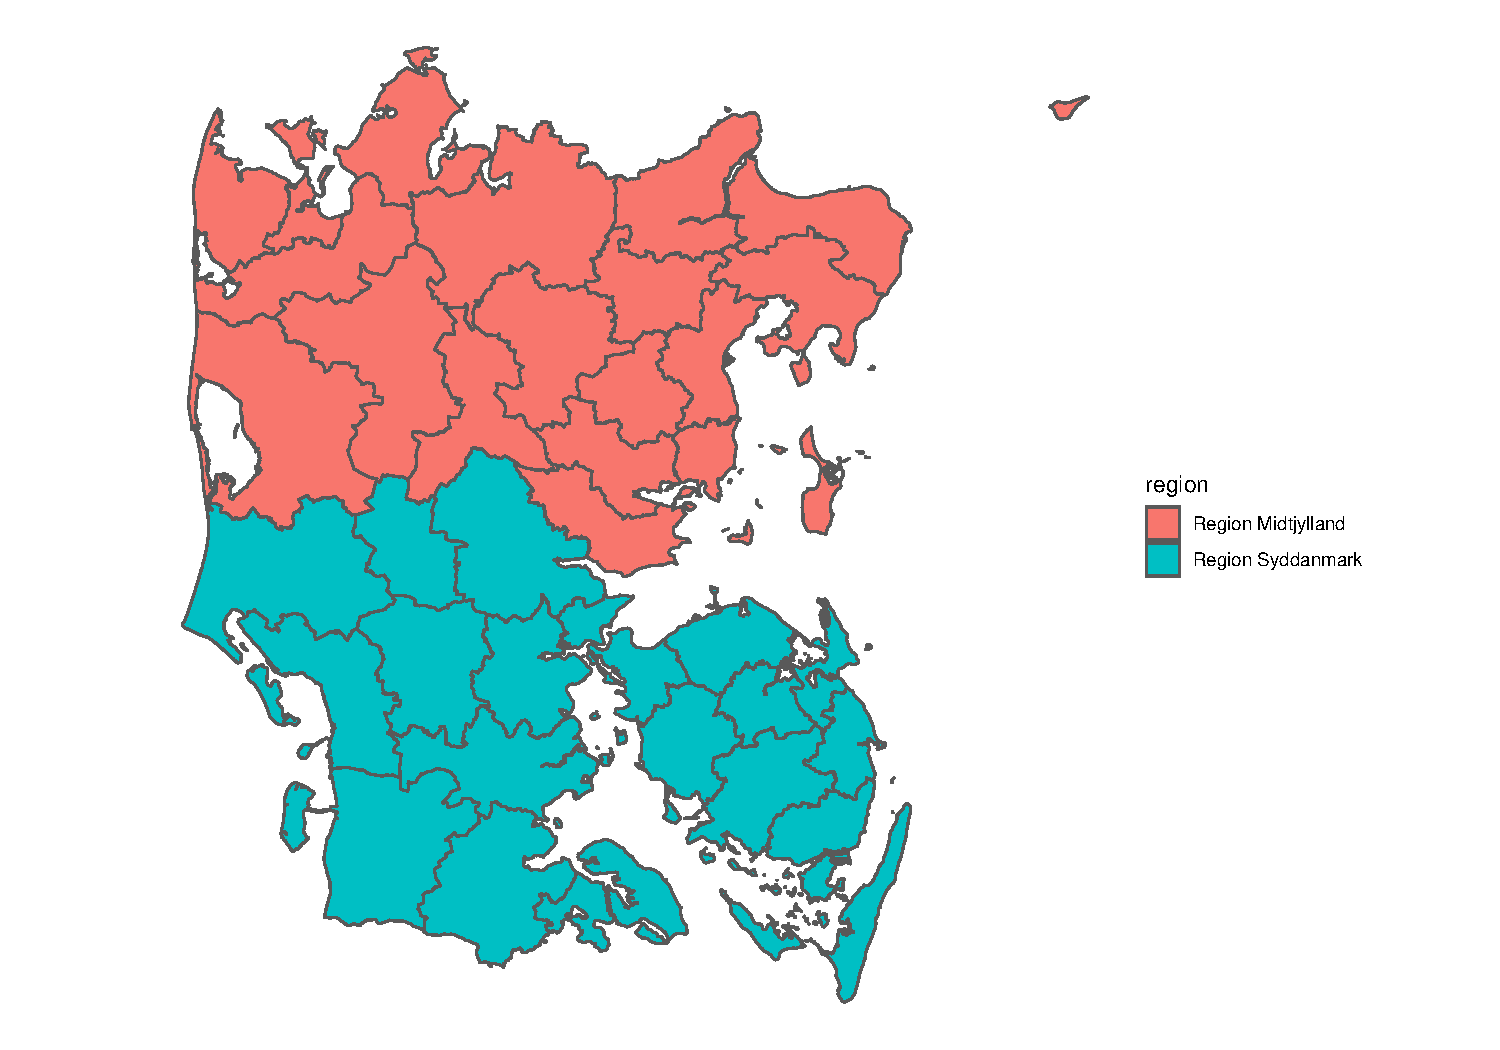
\includegraphics[width=1\linewidth]{crashcourse_slides_files/figure-beamer/unnamed-chunk-7-1}

\columnsend
\end{frame}

\begin{frame}{(3) Polygoner}
\protect\hypertarget{polygoner}{}
\columnsbegin
\column{.4\textwidth}

\begin{itemize}
\item
  Polygoner består -- ligesom linjer -- af punkter, der er kombineret
  til en \emph{polygon} vha. en defineret rækkefølge. Igen, det er
  sjældent noget, I skal bekymre jer om
\item
  Forskellen er, at polygoner er \emph{lukkede linjer}, der former et
  afgrænset område
\item
  De kan have alle tænkelige former. Det centrale er, at polygoner har
  et \emph{areal}
\item
  Eksempler: stater, kommuner, valgkredse osv.
\end{itemize}

\column{.6\textwidth}

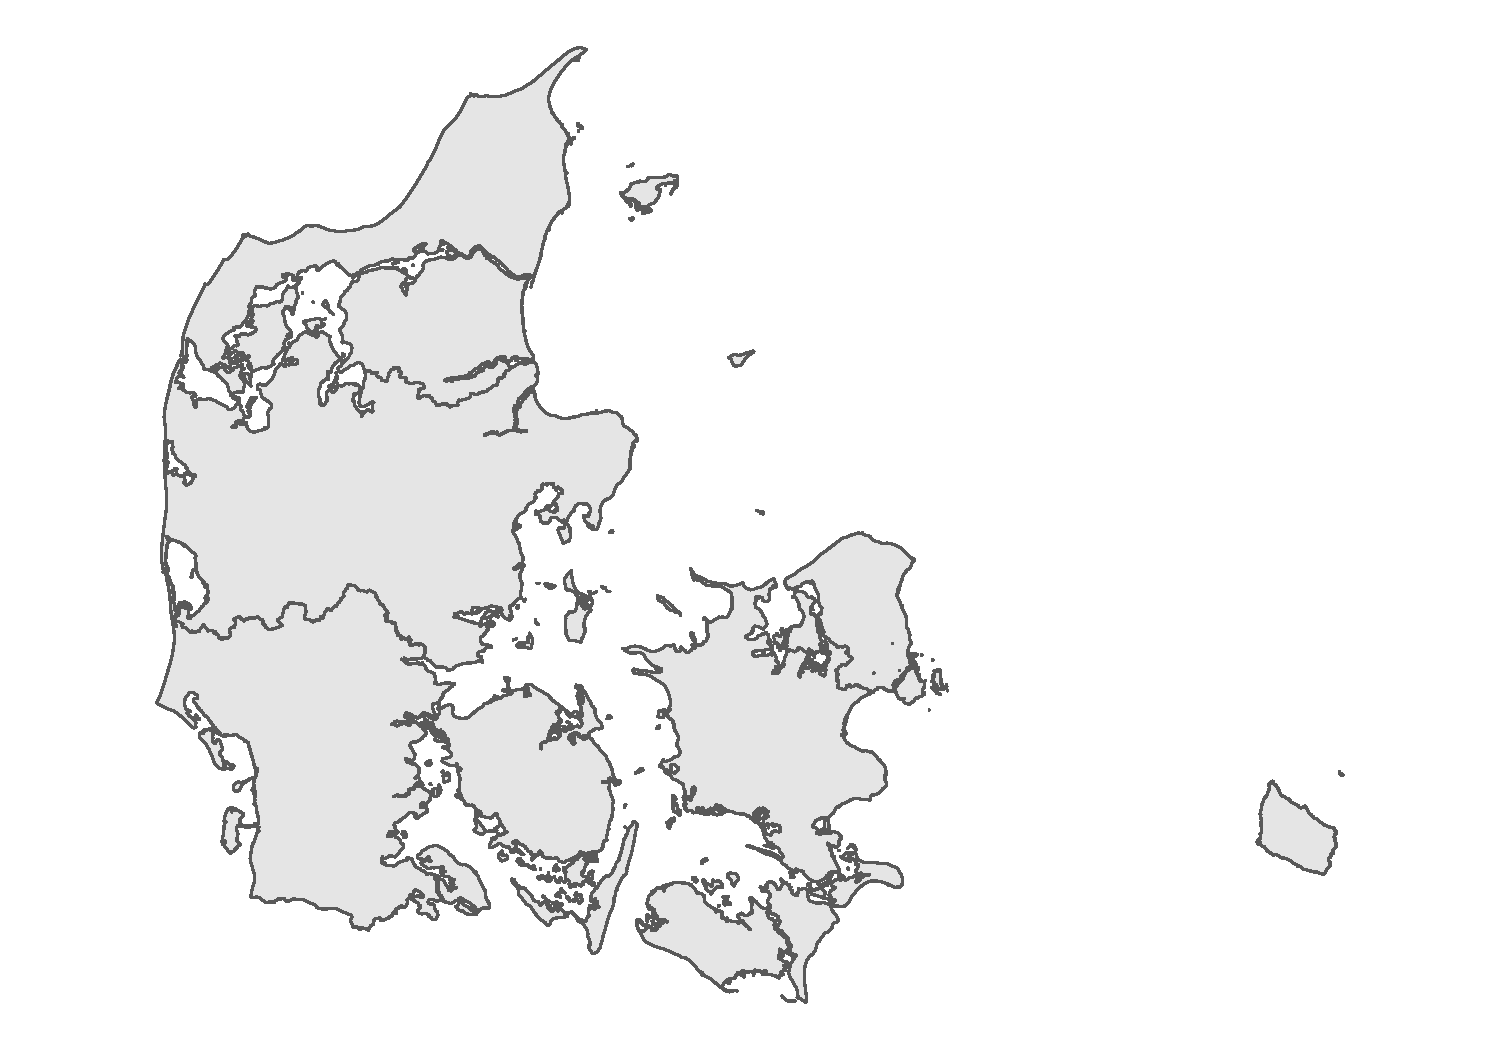
\includegraphics[width=1\linewidth]{crashcourse_slides_files/figure-beamer/unnamed-chunk-8-1}

\columnsend
\end{frame}

\hypertarget{datakilder}{%
\section{Datakilder}\label{datakilder}}

\begin{frame}{DAGI}
\protect\hypertarget{dagi}{}
\columnsbegin

\column{.6\textwidth}

\begin{itemize}
\tightlist
\item
  \emph{``\textbf{Danmarks Administrative Geografiske Inddeling (DAGI)}
  beskriver landets administrative og geografiske inddeling i kommuner,
  regioner, sogne, retskredse, politikredse, postnumre,
  opstillingskredse og lignende.''} --
  \href{https://dawadocs.dataforsyningen.dk/dok/dagi}{DAWA}
\end{itemize}

\medskip

\begin{itemize}
\item
  \ldots{} med andre ord; alt hvad vi kunne drømme om
\item
  DAGI-data kan hentes via Styrelsen for Dataforsyning og
  Effektiviserings
  \href{https://datafordeler.dk/dataoversigt/}{Datafordeler}
\item
  Det er en ret håbløs hjemmeside, til gengæld er der masser at vælge
  mellem (inkl. historiske enheder!)
\end{itemize}

\column{.4\textwidth}

\begin{figure}[H]
    \centering
    
\includegraphics[width=.90\textwidth]{pictures/logo_sdfe.png}
\end{figure}

\columnsend
\end{frame}

\begin{frame}{DAGI}
\protect\hypertarget{dagi-1}{}
\begin{itemize}
\item
  Til de fleste formål kan vi hoppe uden om Datafordelen ved at bruge
  \href{https://dawadocs.dataforsyningen.dk/dok/dagi}{DAWA (Danmarks
  Adressers Web API)} og den
  \href{https://dawadocs.dataforsyningen.dk/dok/api\#dagi}{tilhørende
  API}
\item
  API'en er plug 'n play, hvor vi kan vælge de
  \textcolor{purple}{enheder}, vi skal bruge, og specificere
  \textcolor{teal}{format}:
\item
  \nolinkurl{https://api.dataforsyningen.dk/ \textcolor{purple}{kommuner}?format=\textcolor{teal}{geojson}}
\end{itemize}
\end{frame}

\begin{frame}[fragile]{DAGI: et eksempel}
\protect\hypertarget{dagi-et-eksempel}{}
\columnsbegin
\column{.55\textwidth}

\begin{Shaded}
\begin{Highlighting}[]
\CommentTok{\# definér data}
\NormalTok{url }\OtherTok{\textless{}{-}} 
  \StringTok{"https://api.dataforsyningen.dk/kommuner?format=geojson"}

\CommentTok{\# indlæs data}
\NormalTok{kommuner }\OtherTok{\textless{}{-}} 
  \FunctionTok{read\_sf}\NormalTok{(url)}

\CommentTok{\# plot data}
\FunctionTok{ggplot}\NormalTok{() }\SpecialCharTok{+}
  \FunctionTok{geom\_sf}\NormalTok{(}\AttributeTok{data =}\NormalTok{ kommuner) }\SpecialCharTok{+}
  \FunctionTok{epitheme\_map}\NormalTok{()}
\end{Highlighting}
\end{Shaded}

\column{.45\textwidth}

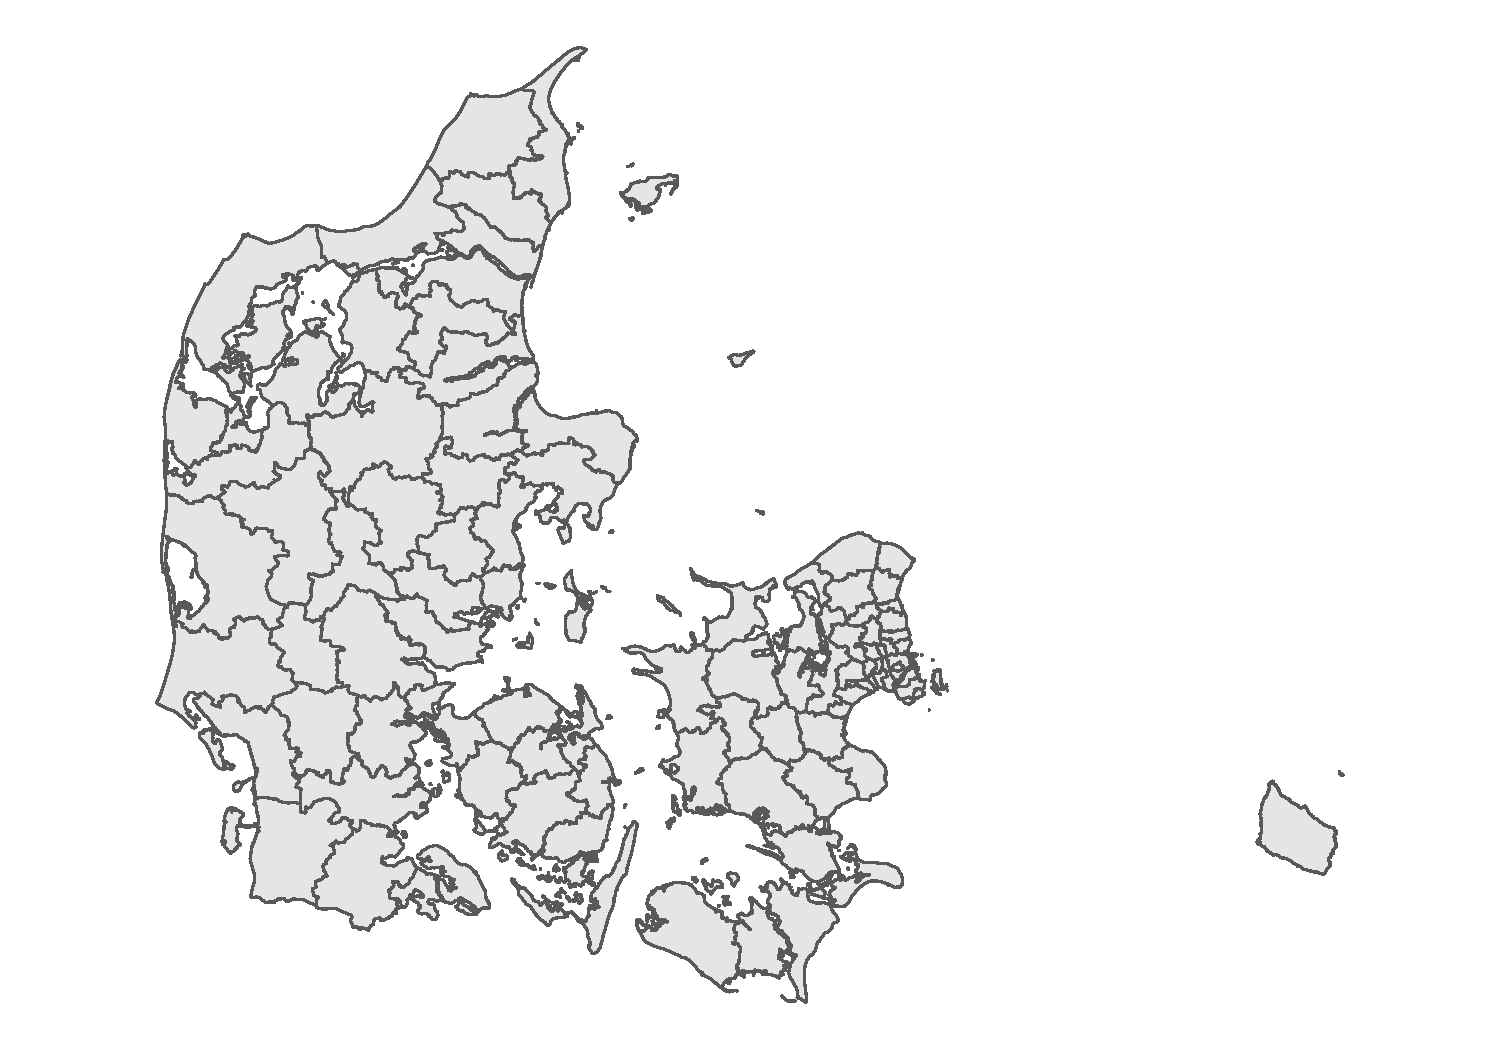
\includegraphics{crashcourse_slides_files/figure-beamer/unnamed-chunk-10-1.pdf}
\columnsend
\end{frame}

\begin{frame}{OpenStreetMap}
\protect\hypertarget{openstreetmap}{}
text \href{https://www.openstreetmap.org/about}{link}
\end{frame}

\hypertarget{indflyvning-til-vuxe6rktuxf8jer-i-r}{%
\section{\texorpdfstring{Indflyvning til værktøjer i
\texttt{R}}{Indflyvning til værktøjer i R}}\label{indflyvning-til-vuxe6rktuxf8jer-i-r}}

\begin{frame}{text}
\protect\hypertarget{text}{}
xx
\end{frame}

\end{document}
